\documentclass[14pt, a4paper]{extarticle}
\usepackage[T2A]{fontenc}
\usepackage[utf8]{inputenc}
\usepackage[english, russian]{babel}
\usepackage{indentfirst, microtype, listings}
\usepackage[unicode, colorlinks=true, allcolors=black]{hyperref}
\usepackage{setspace}
\usepackage{graphicx}
\graphicspath{{images/}}
\usepackage{xcolor} % Подстветка ^_^
\lstset{
    basicstyle=\small\ttfamily,
    columns=fullflexible,
    frame=tb, % draw a frame at the top and bottom of the code block
    tabsize=1, % tab space width
    showstringspaces=false, % don't mark spaces in strings
    numbers=left, % display line numbers on the left
    commentstyle=\color{green}, % comment color
    keywordstyle=\color{blue}, % keyword color
    stringstyle=\color{red} % string color
}
\usepackage[left=2cm, right=2cm, top=2cm, bottom=2cm]{geometry}
\newtheorem{definition}{Определение}


\begin{document} % Начало документа
    \begin{titlepage}
        \begin{center}
            МИНОБРНАУКИ РОССИИ

            ФЕДЕРАЛЬНОЕ ГОСУДАРСТВЕННОЕ БЮДЖЕТНОЕ

            ОБРАЗОВАТЕЛЬНОЕ УЧРЕЖДЕНИЕ

            ВЫСШЕГО ОБРАЗОВАНИЯ

            «ВОРОНЕЖСКИЙ ГОСУДАРСТВЕННЫЙ УНИВЕРСИТЕТ»

            \begin{spacing}{4}
            \end{spacing}

            Математический факультет
            \begin{spacing}{5.5}
            \end{spacing}


            Клиент-серверное приложение для управления персоналом и проектами
            \begin{spacing}{4.5}
            \end{spacing}


            Выпускная квалификационная работа 

            «Системный инженер (специалист по эксплуатации аппаратно-программных комплексов персональных ЭВМ и сетей на их основе)»

        \end{center}

        \begin{spacing}{5.5}
        \end{spacing}

        Допущено к защите в ИАК	 10.06.2019

        \begin{spacing}{2}
        \end{spacing}

        \begin{spacing}{2}
        \end{spacing}
        Обучающийся \def\hrf#1{\hbox to#1{\hrulefill}}
        \hrf{5em} А.А. Уткин
        \begin{spacing}{2}
        \end{spacing}
        Руководитель\ \ \def\hrf#1{\hbox to#1{\hrulefill}}
        \hrf{5em}
                профессор Костин Д.В.

        \begin{center}
            \begin{spacing}{4}
            \end{spacing}
            Воронеж 2019
        \end{center}
    \end{titlepage}
    % Начало оглавления. Оно хитро заполняется само, глядя на заголовки
    % которые добавляются с помощью \section и \subsection
    \renewcommand\contentsname{Оглавление} %%% renaming the Table of Contents
    \tableofcontents
    \setcounter{page}{2}

    \pagebreak
    \section*{Введение}
    % Такой заголовок пойдет в оглавление, только без нумерации
    \addcontentsline{toc}{section}{Введение}


    \clearpage
    \section{Постановка задачи}

    Принцип действия вибрационного погружателя основан на эффекте резкого снижения сопротивлению погружения свайного элемента при сообщении последнему вибрации. При вращении дисбалансов на их ось крепления действует центробежная сила и вибрационный погружатель получает вибрирующее движение, которое сообщается свайному элементу через наголовник.

    \begin{definition}
        Вибрационным погружением называют внедрение твёрдого тела в сопротивляющуюся среду под действием постоянной и знакопеременной сил.
    \end{definition}
    
    \begin{definition}
        Под вибрационным внедрением будем понимать внедрение твёрдого тела в сопротивляющуюся среду с заданной средней скоростью.
    \end{definition}

    \begin{definition}
        Дебалансом называют неуравновешенность вращающихся частей машин (роторов, коленчатых валов, шкивов и т. п.).
    \end{definition}

    \begin{figure}[h]
        \centering
        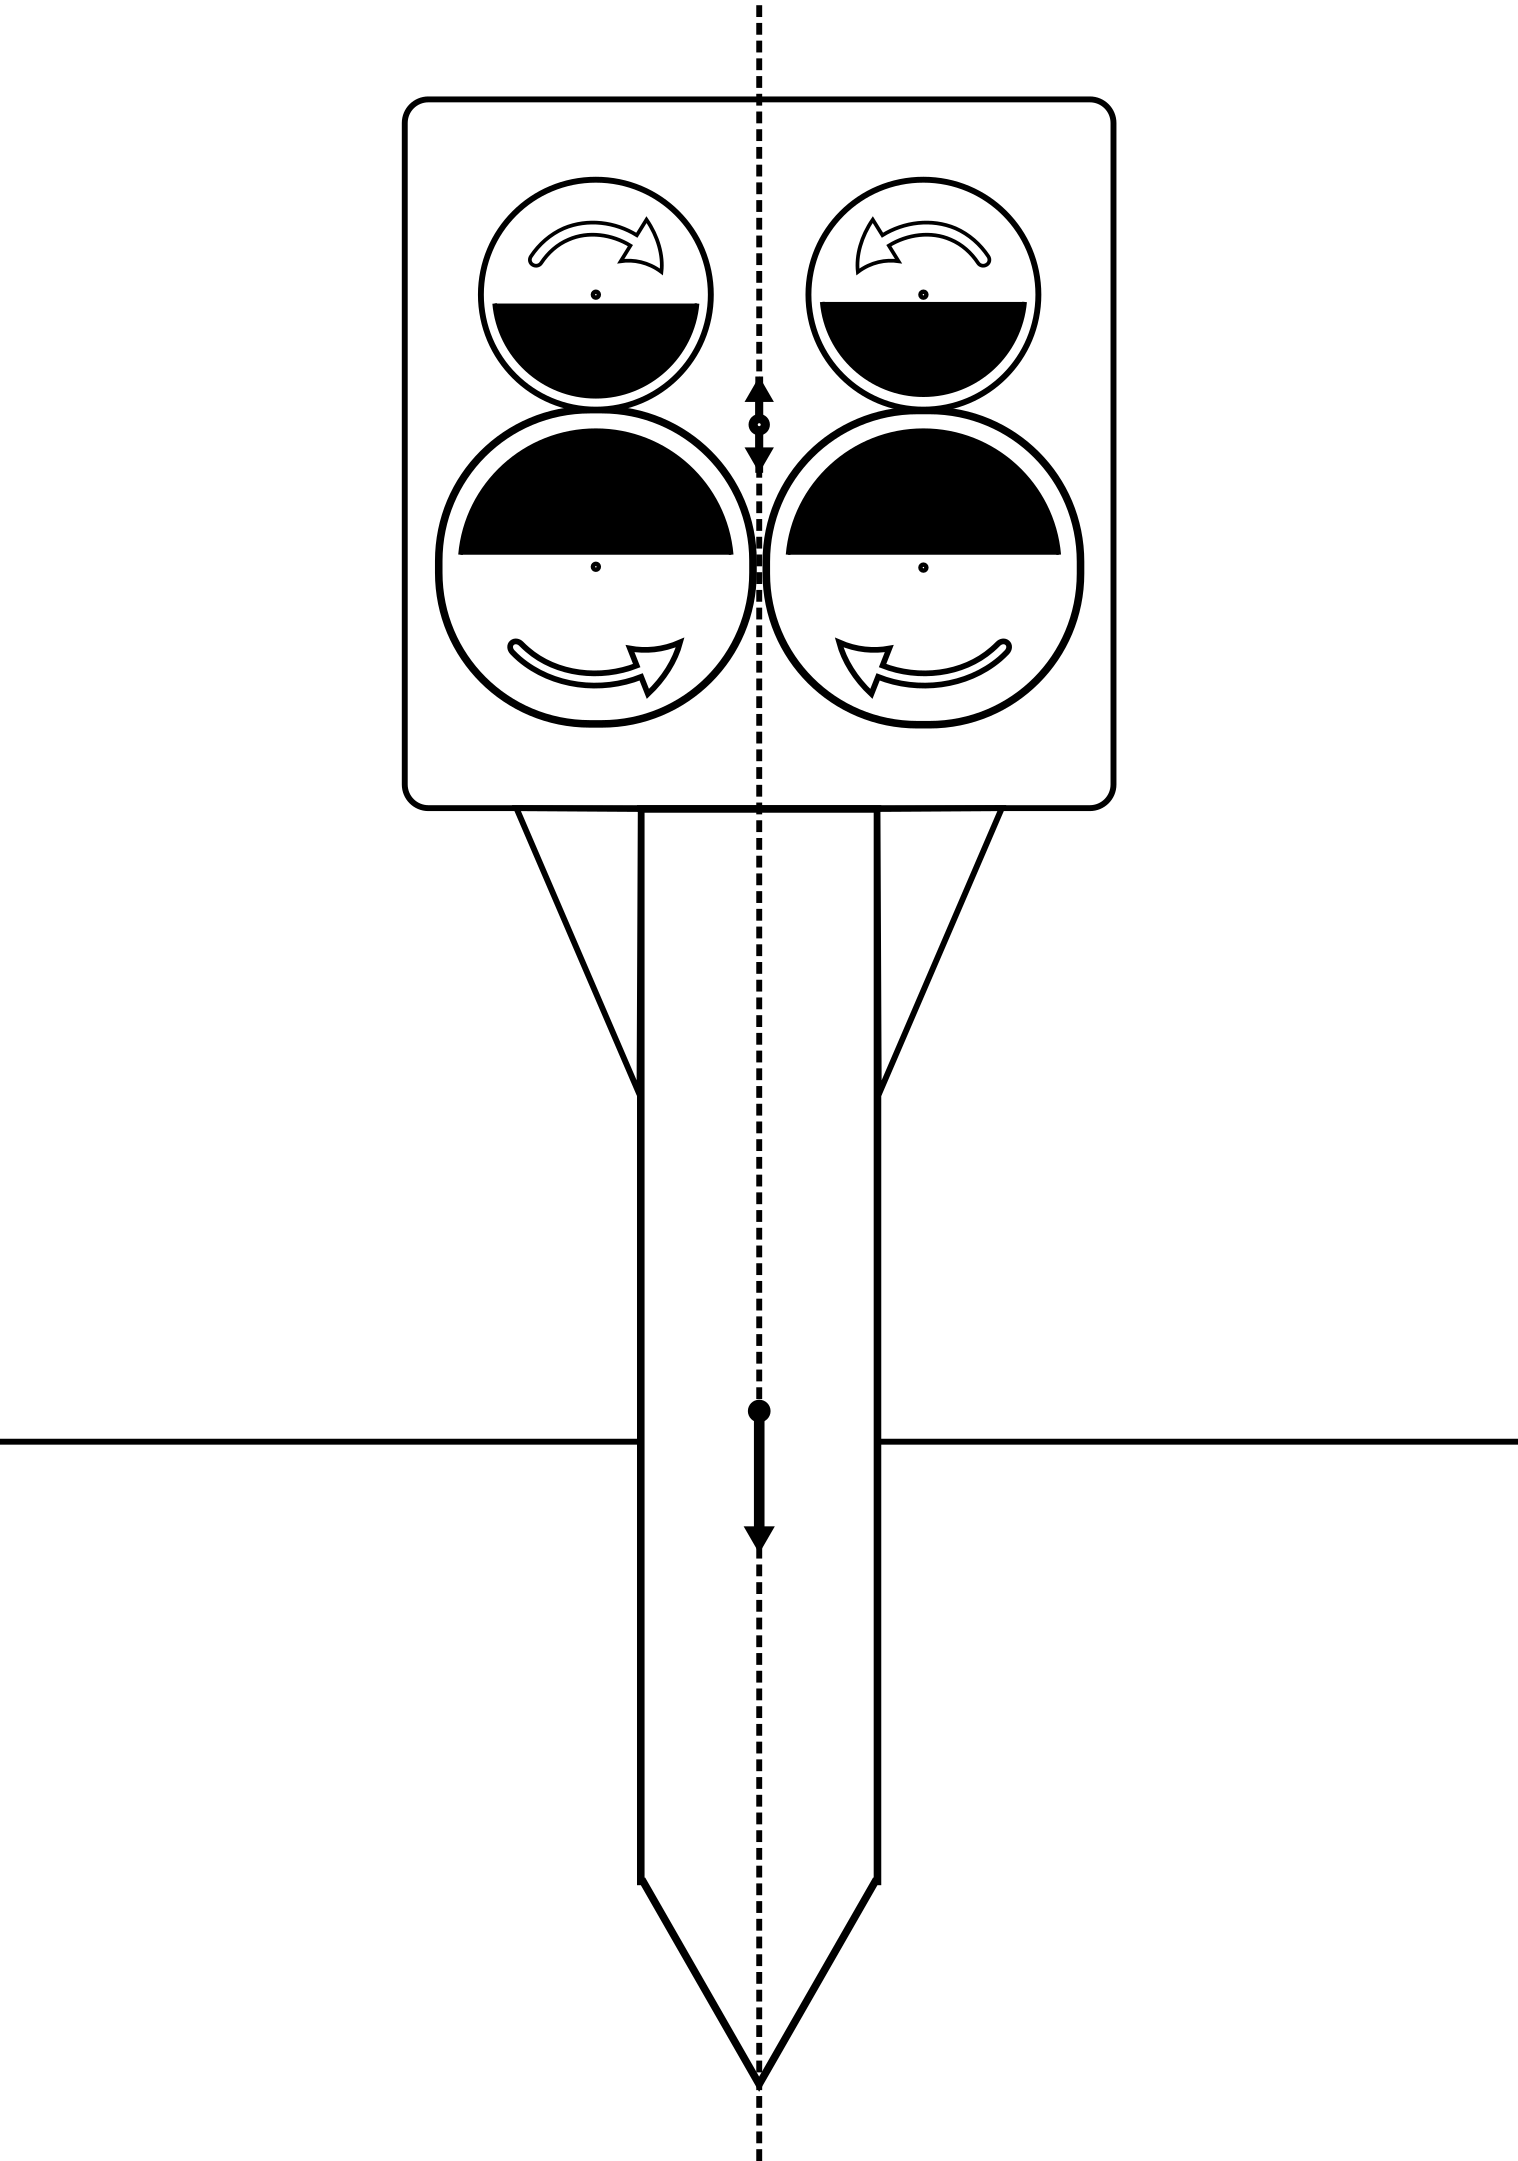
\includegraphics[width=0.5\linewidth]{img/scheme_porg.png}
        \caption{Схема вибрационного погружателя.}
        \label{fig:scheme_porg}
    \end{figure}

    \begin{definition}
        Сила, препятствующая материальной точке, движущейся по окружности, удалиться от центра этой окружности, называется центростремительной силой. Она направлена по радиусу от окружности к центру. По третьему закону Ньютона имеется равная ей и противоположно направленная сила противодействия (сила, с которой движущаяся точна стремится удалиться от центра). Эта сила называется центробежной.
    \end{definition}
    
    \clearpage
    \section{Заключение}


    \clearpage
    \section{Приложение}
    \subsection{Исходный код main.py}
    % \lstinputlisting[language=Python, breaklines]{code/app.py}


    \clearpage
    \addcontentsline{toc}{section}{Список литературы}
    \begin{thebibliography}{}
        \bibitem{}
    \end{thebibliography}
\end{document}
